% Jeg tror det er tre spørsmål som kan besvares her:
% 1. Hvor mye enklere/bedre er det å utvikle apps med Kvik microservices?
% 2. Overhead/ improvement for enkelt-microservices. Dvs overhead for de som
% tilbyr noe mer en alternativet (container tilbyr enklere deployment men har en
% overhead på...), og improvement for de som optiamliserer noe (Kvik vs OpenCPU,
% eventuelt begge deler (caching for MsigDB reduserer query tid men har en
% storage overhead)
% 3. Performance analyse av MIxT. Hvor er det overheadene er for en query? Overhead for mange samtidige queries?
%
% Metodologi:
% 1. Kvik-MIxT vs 1000-R-linjer-MIxT? Og kanskje anektdoter som at container
% kunne flyttes til AWS. Eller noe helt annet.
% 2. En av de enklere web apps som er laget før. Eventuelt en benchmark app.
% 3. MIxT operasjoner.
%
We show the viability of the microservices approach in Kvik by describing the
MIxT web application for exploring and comparing
transcriptional profiles from blood and tumor samples. 

Figure \ref{kvik-mixt} shows the relationship between MIxT and Kvik. MIxT
consists of a web application and an R package, while Kvik provides the services
for doing database lookup of genes and processes, as well as executing
statistical analyses. 


\begin{figure}[h!]
\centering
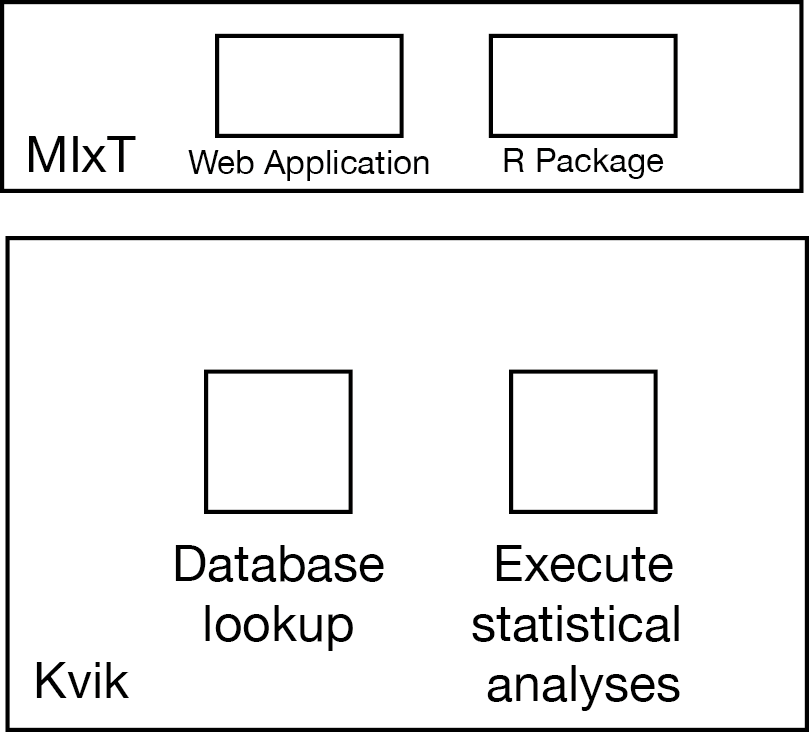
\includegraphics{figures/kvik-mixt.png}
\caption{An overview of the relationship between the MIxT application and Kvik.
MIxT contains a web application (online at \url{mixt-blood-tumor.bci.mcgill.ca})
and the R Package that provides analyses and data to the web application. Kvik
provides the services for running the statistical analyses from the R package,
and the database lookups found in the web application.} 
\label{kvik-mixt}
\end{figure} 

% \subsection*{Design} 
We define six data exploration tasks that the web application should help users
perform: 

\textbf{Explore co-expression gene sets in tumor and blood tissue}. We want to
simplify the process of exploring the computed co-expression gene sets, or
modules, through the web-application. The application should 
visualize gene expression together with clinicopathological variables associated
with each module. In addition we want to enable users to study the underlying
biological functions of the modules by including gene set analyses between the
module genes and known gene sets. 

\textbf{Explore co-expression relationships between genes}. Users should be able
to explore the co-expression relationship as a graph visualization. The network
should visualize each gene as a node and a significant co-expression
relationship as an edge.  

\textbf{Explore relationships between modules from each tissue.} Users should be
able to explore the relationship between modules from different tissues. We
provide two different metrics to compare modules, and the web application should
enable users to interactively browse these relationships. In addition to
providing visualizations the compare modules from each tissue, users should also
be able to explore the relationships, but for different breast cancer subtypes. 

\textbf{Explore relationships between clinical variables and modules.} In
addition to comparing the association between modules from both tissues, users
also have the possibility of exploring the association with a module and a
specific clinical variable. This should also be possible for the different
breast cancer subtypes. 

\textbf{Explore association between user-submitted gene lists and computed
modules.} We want to enable users to explore their own gene lists to explore
them in context of
the co-expression gene sets. The web application must handle uploads of gene
lists and compute association on demand. 

\textbf{Search for genes or gene lists of intrest}. To facilitate faster lookup
of genes and processes, the web application should provide a search
functionality that lets users locate genes or gene lists and show association to
the co-expression gene sets. 

% Vi kan godt kutte én av figurene under, f.eks c eller d som er veldig lik. 
\begin{figure*}[h!]
\centering
\caption{MIxT module overview page. The screenshot show the user interface for
exploring a single module. It consists of three panels. The top left panel
contains the gene expression heatmap. The top right panel contains a table of
the genes found in the module. The bottom panel contains the results of gene
overlap analyses from the module genes and known gene sets from MSigDB.}
%\caption{Screenshots of the user interface in four of the six analysis tasks.
%Note that we combine visualization frameworks for both JavaScript and R to
%generate the visualizations. Specifically, sigmajs (a,
%\protect\url{sigmajs.org}), ggplot2(b, \protect\url{ggplot2.org}), and D3 (c and
%d, \protect\url{d3js.org})}
%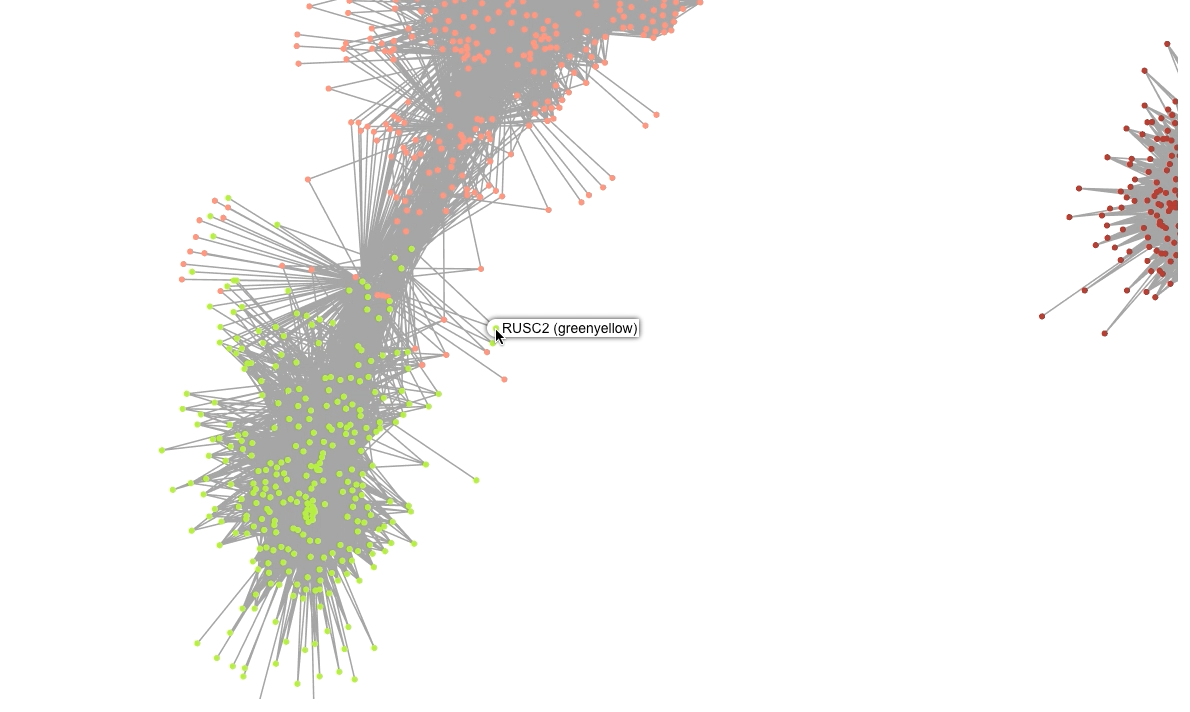
\includegraphics[width=2.7in]{figures/network.png} 
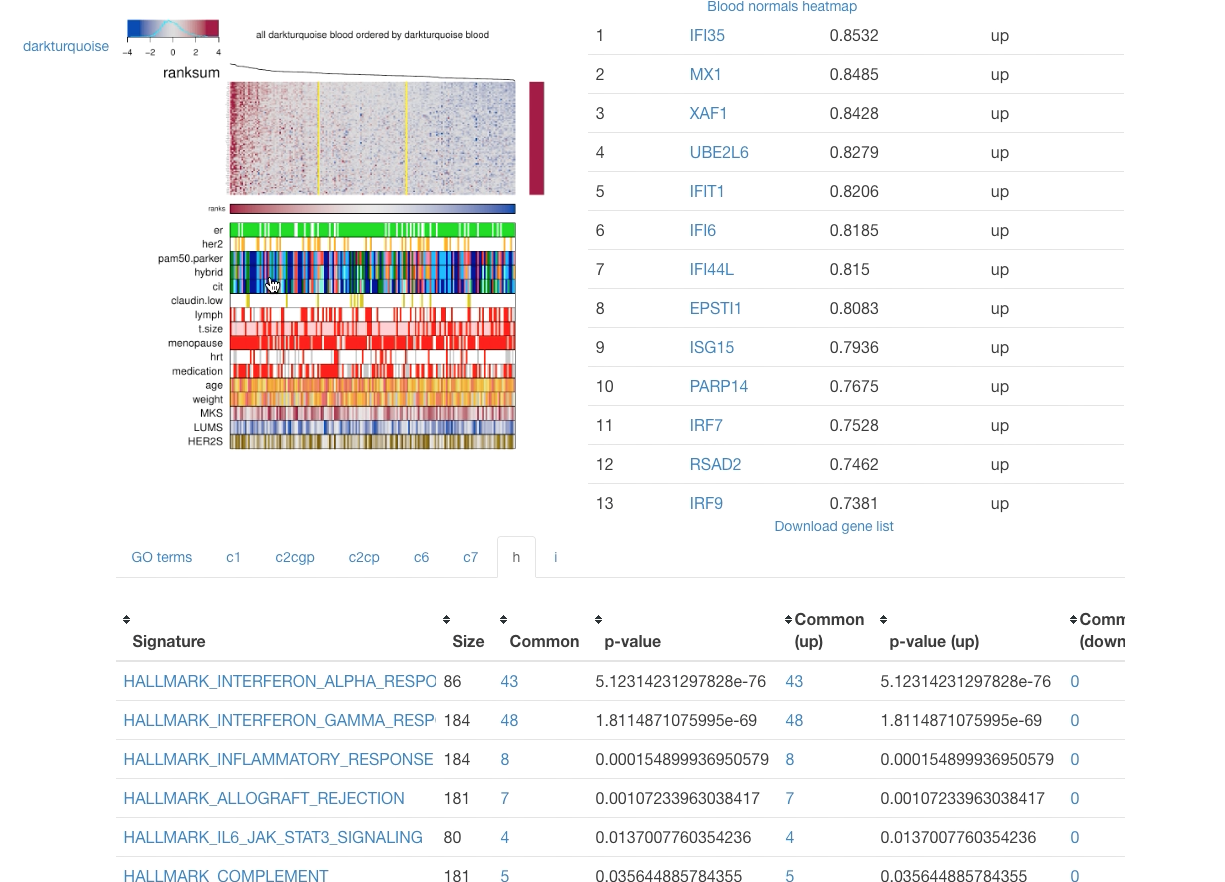
\includegraphics[width=0.8\textwidth]{figures/module.png}
% 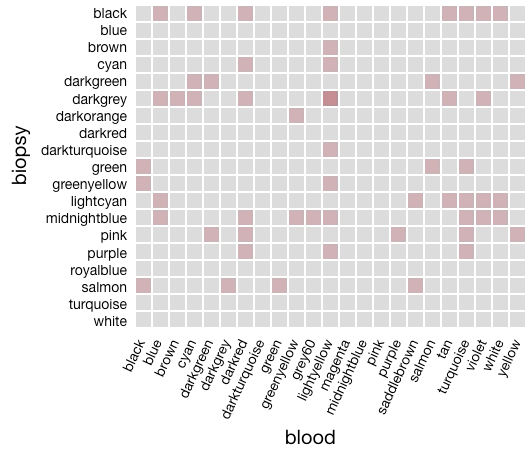
\includegraphics[width=2.5in]{figures/tissue-comp.png}
\label{fig_first_case}
\end{figure*} 

% \hfil
% \subfloat[A2: Module visualization.]{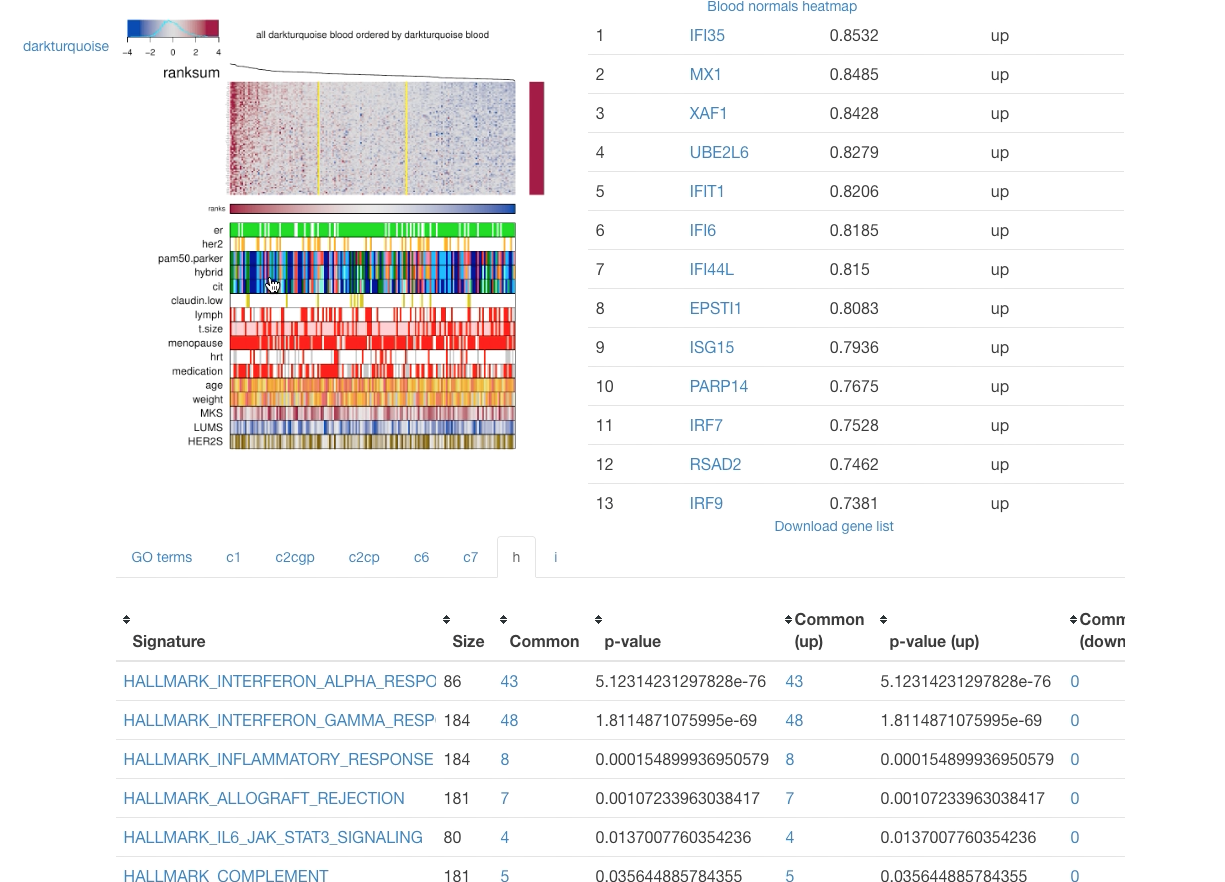
\includegraphics[width=2.5in]{figures/module.png}%
% \label{fig_second_case}}
% \hfil
% \centering
% \subfloat[A3: Visualization of ranksum.]{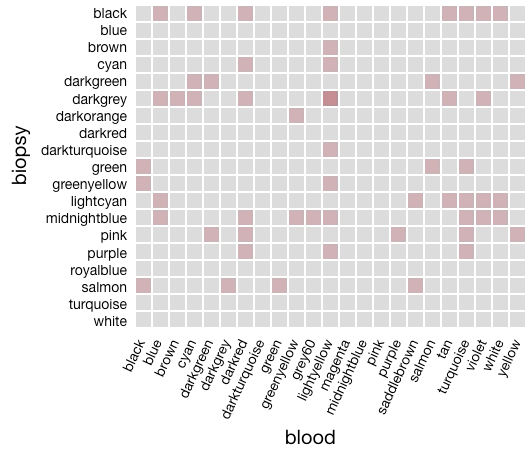
\includegraphics[width=2.5in]{figures/tissue-comp.png}%
% \label{fig_first_case}}
% \hfil
% \subfloat[A4: Visualization of significant clinical variable
% association]{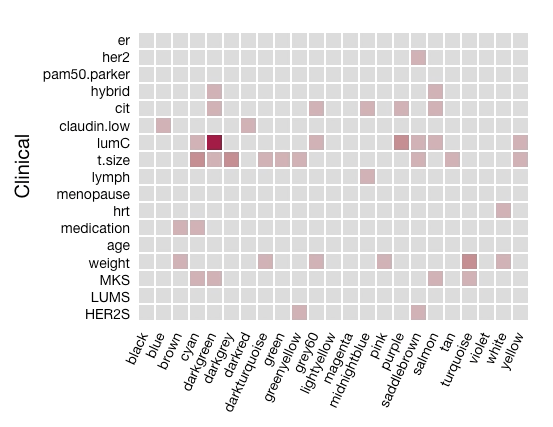
\includegraphics[width=2.8in]{figures/clinical-comp.png}%
% \label{fig_second_case}}
% \caption{Screenshots of the user interface in four of the six analysis tasks.
% Note that we combine visualization frameworks for both JavaScript and R to
% generate the visualizations. Specifically, sigmajs (a,
% \protect\url{sigmajs.org}), ggplot2(b, \protect\url{ggplot2.org}), and D3 (c and
% d, \protect\url{d3js.org})} 
% \label{fig_sim}
% \end{figure*}


From these six analysis tasks we designed and implemented MIxT as a web
application that integrates statistical analyses and information from biological
databases together with interactive visualizations.
The MIxT web application
consists of three services: i) the web application itself containing the
user-interface and visualizations; ii) the compute service performing the MIxT
analyses delivering data to the web application; and iii) the database service
providing up-to-date information from biological databases. Each of these
services run within Docker containers making the process of deploying the
application simple. 
By composing the
application of a set of services we can substitute parts of the application
without re-writing the entire application.
For example if we want to use OpenCPU to interface with data analysis we can do
so by simply exchanging the Kvik compute service with OpenCPU. Both services
communicate over HTTP and their interfaces are the same. 

We structured the MIxT application with a separate view for each analysis task.

To explore the co-expression gene sets we built a view that combines both static
visualizations from R together with interactive tables with gene overlap
analyses. Figure \ref{fig_first_case} shows the web page presented to users when
they access the co-expression gene set 'darkturquoise' from blood. Using the
Kvik compute service we can generate plots on demand and provide users with
high-resolution PDFs or PNG files. 

To explore the co-expression relationship between genes we use an interactive
graph visualization build with Sigmajs\footnote{\url{sigmajs.org}}. We have
built visualization for both tissues, with graph sizes of 2705 nodes and 90 348
edges for the blood network, and 2066 nodes and 50 563 edges for the biopsy
network. The sigmajs visualization library has functionality for generating a
layout for large networks, but we generate this layout server-side to reduce the
computational load on the client. To generate this layout we use the GGally
package\footnote{\url{cran.r-project.org/web/packages/GGally}}. By generating
the network layout using the compute service we relieve the clients.

To visualize relationships between modules from different tissues, or their
relationship to clinical variables we built a heatmap visualization using the 
d3\footnote{\url{d3js.org}} library. Figure \ref{fig_second_case} shows an
example of this heatmap visualization, showing the association between the
clinical variables and the modules from biopsy for all samples.  

\begin{figure}[h!]
\centering
\caption{Heatmap visualization of the association between clinical variables and
the modules in biosy. The visualization is built using the d3 JavaScript
library.} 
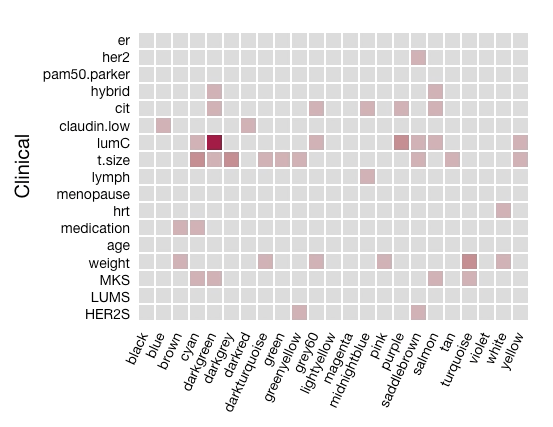
\includegraphics[width=2.5in]{figures/clinical-comp.png}
\label{fig_second_case}
\end{figure} 
